\documentclass[11pt,a4paper]{article}

\usepackage[margin=1in]{geometry}
\usepackage{amsmath,amssymb,amsthm,mathtools}
\usepackage{booktabs}
\usepackage{graphicx}
\graphicspath{{charts/}{./}}
\usepackage{hyperref}
\hypersetup{colorlinks=true,linkcolor=blue!60!black,urlcolor=blue!60!black,citecolor=blue!60!black}

\theoremstyle{plain}
\newtheorem{theorem}{Theorem}
\newtheorem{proposition}{Proposition}
\newtheorem{lemma}{Lemma}
\newtheorem{corollary}{Corollary}
\newtheorem{definition}{Definition}
\theoremstyle{remark}
\newtheorem{remark}{Remark}

\title{The Curved-Corpus Program, Unified:\\
{\large Learned Latent Curves, a Null-Standardized Question Space, and Spherical Defocus,\\ with Machine-Checked Invariants}}
\author{Shant Tchatalbachian}
\date{August 13, 2026 (v1) --- revised August 22, 2026 (v2)}

\begin{document}
\maketitle

\begin{abstract}
This paper merges the two prior papers of the curved-corpus program --- \emph{Learned Latent Curves and the Hyperspherical-Harmonic} (2026-08-06) and \emph{Is This $X$?} (2026-08-12) --- into one account, and extends the merged framework in three directions. (i) \textbf{An optical reading with exact anchors.} The M\"obius chart $\varphi_\theta\in\mathrm{PSL}(2,\mathbb{C})$ carried (frozen at identity) through every prior run is precisely the object of Leonhardt's optical conformal mapping, with index profile $n(z)=|\varphi_\theta'(z)|$; the single-action atom's geodesic-only criterion is a discrete Fermat principle; null standardization is the statistical analogue of measuring lensing deflection against an unlensed background, with the fixed-margin ensemble as the medium (Lyu--Mukherjee give its spectrum analytically) and $\Delta V_2=+0.0144$ at $z=+12.3$ as the deflection; and the program's exact-$1.0000$ gate passes are caustics --- rank degeneracies where over-focusing destroys data content. (ii) \textbf{Spherical defocus (experiment G1, executed).} The 16 real spherical harmonics of $L=3$ are eigenfunctions of the Laplace--Beltrami operator, so Brownian motion on $S^2$ acts diagonally on the program's own basis. The semigroup identity $\mathbb{E}[Y_{\ell m}(B_t^x)]=e^{-\ell(\ell+1)t}Y_{\ell m}(x)$ is verified by simulation on a Fibonacci lattice ($N{=}2048$, measured/predicted ratios $1.000$--$1.028$ across $t\in[0.01,0.2]$, $\ell\in\{1,2,3\}$). On the real $2286\times9$ corpus the closed-form decay does \emph{not} govern point diffusion: per-degree energies collapse by $60$--$90\%$ at $t=0.005$ where the closed form predicts $\le6\%$, non-monotonically in $\ell$, because the corpus is atomic ($176$ distinct rows of $512$); the gap is promoted to an \emph{atomicity diagnostic} $A_\ell(t)$, and the null space acquires an exact dynamical meaning as the $t\to\infty$ endpoint of the forward heat flow. Geodesic (slerp) interpolation is identified as the deterministic half of the sphere Langevin step whose zero-temperature limit is the historical absorbing edit log, extending the curve-compass $\pm$ atom from the ten $k$-shells to the full sphere. (iii) \textbf{Machine-checked invariants.} The program's identity-type claims --- the atom invariant $\Delta\ge0$, linear composition, cumulative monotonicity, the gate--rank equivalence $V_2\ge0.40\iff\hat r\le5$, the $\Phi$-ladder telescoping identity, monotonicity and additivity of the heat exponent $\ell(\ell+1)$, and the $\min$-symmetry at the core of Metropolis--Hastings detailed balance --- are formalized and proved in Lean~4 (core toolchain, no \texttt{mathlib}), so the boundary the program draws between identities and measurements is now itself machine-checked. All prior corrections, retractions, and honesty constraints are carried forward unmodified.
\end{abstract}

\section{Introduction}
\label{sec:intro}

The curved-corpus program has produced two papers and a running argument between them. The first (Tchatalbachian, 2026a) built the instrument: a family of learned latent curves on $[0,1]$ and on the Riemann sphere $S^2$, a single-action audit atom with an only-positive-$\Delta$ invariant, and a recursive improvement loop that drove three corpora to full primitive coverage across $1391$ dispatches with zero regressions. The second (Tchatalbachian, 2026b) audited the instrument: it showed the headline observable $V_2=\mathrm{PC1}+\mathrm{PC2}$ is $98\%$ fixed by marginals, that its celebrated transition was a basis change, that its gate is a rank test a noise corpus passes exactly, retracted the program's most-cited intermediate correction, inverted the Hodge reading (the corpus is anti-cyclic), and replaced the sequence of candidate $X$'s with a null-standardized question space issuing exclusion-only verdicts.

This paper does three things. First, it \textbf{merges} the two accounts into one, keeping the second paper's corrections as binding on the first's claims (Sections~\ref{sec:family}--\ref{sec:audit}). Second, it adds an \textbf{optical reading} with exact rather than metaphorical anchors, and uses it to organize a chain the program has been circling: question space $\to$ intent space $\to$ null space $\to$ latent space of $0$ through $N$ dimensions (Section~\ref{sec:optics}). Third, it opens a \textbf{diffusion channel}: geodesic (slerp) interpolation on the hypersphere generates a Brownian defocus that is diagonal in the program's own harmonic basis, and experiment G1 --- executed here --- verifies the governing semigroup identity on the sampling lattice and measures its instructive failure on the real corpus (Section~\ref{sec:defocus}). A short section records which of the program's statements are identities and proves them in Lean~4 (Section~\ref{sec:lean}); scope and caveats close (Section~\ref{sec:scope}).

Two disciplines are inherited verbatim from the 2026-08-12 paper: no statistic is reported without its matched null, and no coordinate is admitted to the map without a demonstrated non-degenerate null. The optical and diffusion vocabulary introduced here is held to the same bar: each term is used only where a metric and a variational problem are both specified, and each proposed coordinate arrives with the null it must pass before admission.

\section{The curve family}
\label{sec:family}

\subsection{Flat curve, ridge, gate}
For output dimension $j=1,\dots,D$ and ordering coordinate $t\in[0,1]$,
\begin{equation}
z_j(t)=a_{j,0}+\sum_{m=1}^{k}\big(a_{j,m}\sin(2\pi f_mt)+b_{j,m}\cos(2\pi f_mt)\big),\tag{1}
\end{equation}
with $k$ shared learned frequencies; stacking the design vector $\phi(t)$ gives $\gamma(t)=C\phi(t)$, solved at fixed frequencies by the Tikhonov ridge
\begin{equation}
C^{\star}=(\Phi^{\top}\Phi+\lambda I)^{-1}\Phi^{\top}Z,\qquad\lambda=10^{-3}.\tag{2}
\end{equation}
The coordinate $t$ is the rank of the top principal component of the $z$-scored feature matrix, and the fit gate is
\begin{equation}
V_2=\mathrm{PC1}+\mathrm{PC2}=\frac{\lambda_1+\lambda_2}{\sum_{a=1}^{D}\lambda_a}\ \ge\ 0.40 .\tag{3}
\end{equation}

\subsection{Hyperspherical variant, M\"obius chart, Fibonacci sampling}
For $\mathbf{x}\in S^2$,
\begin{equation}
\gamma(\mathbf{x})=\mathbf{b}+\sum_{\ell=0}^{L}\sum_{m}\mathbf{a}_{\ell,m}\,Y^{S^2}_{\ell,m}\!\big(\varphi_\theta(\mathbf{x})\big),\qquad n_{\mathrm{basis}}=16\ \text{at}\ L=3,\tag{4}
\end{equation}
with the M\"obius reparameterization $\varphi_\theta(z)=(az+b)/(cz+d)$, $ad-bc=+1$, six real degrees of freedom, \emph{frozen at the identity in every run reported to date}. Items reach $S^2$ by the stereographic lift $\sigma(u,v)=(2u,2v,u^2+v^2-1)/(1+u^2+v^2)$ of their PCA top-2 coordinates. Sampling uses Vogel's golden-angle lattice
\begin{equation}
z_i=1-\tfrac{2i+1}{N},\qquad\phi_i=2\pi i/\varphi_g,\qquad\theta_i=\arccos z_i,\qquad\varphi_g=\tfrac{1+\sqrt5}{2},\tag{5}
\end{equation}
under which the Gram matrix of the 16 real harmonics is near-orthonormal, $B^{\top}B\approx(N/4\pi)I_{16}$, condition number $1.003$--$1.006$ in every design of this program.

\subsection{The single-action atom}
The smallest audit unit maps a file to one point $p\in S^2$ (coverage vector $\to$ PCA top-2 $\to$ lift), defines the ideal pole $p^*$ as the lift of the all-ones vector, the geodesic gap $d(f)=\|p-p^*\|_2$, and selects among single missing-primitive flips the one minimizing post-flip distance.

\begin{lemma}[atom invariant]
\label{lem:atom}
For any file $f$ and any action selected by the geodesic-only criterion, $\Delta_f=d_{\mathrm{pre}}-d_{\mathrm{post}}\ge0$.
\end{lemma}

\begin{theorem}[linear composition]
\label{thm:comp}
For a corpus of $N$ files with atomic actions $\alpha_1,\dots,\alpha_N$, $\Delta_{\mathrm{corpus}}=\sum_i\Delta_{f_i}$; if every atomic $\Delta\ge0$ then $\Delta_{\mathrm{corpus}}\ge0$.
\end{theorem}

\begin{corollary}[cumulative monotonicity]
\label{cor:mono}
The running total over cycles is monotone non-decreasing; the per-cycle increment is unconstrained in shape.
\end{corollary}

Empirically: $1391$ dispatches over three corpora (\texttt{skills/} $474$, \texttt{docs/} $126$, \texttt{refs/} $791$), $598$ strictly positive $\Delta$, zero negative, cumulative $\Delta=+59.7671$, all three corpora absorbing at full coverage; the realized $\Delta$ depends only on the missing-primitive count $k$, unimodal with peak at $k=5$ ($\Delta=0.1206$), identically on all three corpora. The matched-parameter ablation favors the sphere over a capacity-matched flat Fourier baseline ($49$-item $\delta=+0.977$; $70$-item $\delta=+1.342$; single-seed point estimates), and the synthetic-manifold benchmark holds both controls (torus: flat wins $50/50$ seeds, $p<10^{-15}$; sphere: sphere wins $50/50$, $p<10^{-55}$). Section~\ref{sec:lean} formalizes all three statements above.

\section{The audit, carried forward}
\label{sec:audit}

The corrections of the 2026-08-12 paper are restated here as binding, in compressed form; every number is from the shipped evidence bundle and its reproduction manifest.

\textbf{C1 (dimension artifact).} $V_2$ is a trace-normalized share and decays in $D$ at fixed rows (flat-spectrum floor $2/D$); on identical $2286$ rows, $V_2=0.7235$ at $D=9$ and $0.2940$ at $D=24$. The celebrated $+0.4664$ ``transition'' was this proposition evaluated at two points.

\textbf{C2 (the gate is a rank test).} The shipped estimator reports $\hat r=2/V_2$, so $V_2\ge0.40\iff\hat r\le5$ is a definitional identity (formalized in Section~\ref{sec:lean}); the $(\ell{=}384,m{=}3)$ variant and 2-D PCA return exactly $1.0000$ on all six corpora including single-class iid noise. Exact $1.0000$ is a red flag; Section~\ref{sec:optics} gives it a geometric name.

\textbf{C3 (corrected null, and a retraction).} Under the fixed-margin curveball null (two independently validated uniform samplers), the $2286\times9$ matrix has null $V_2=0.709180\pm0.001183$ against real $0.723529$: $\Delta V_2=+0.0144$, $z=+12.13$, $\mathbb{E}_0[V_2]/V_2=0.9802$. The intermediate value $0.8005$ ($z=-45.8$) is retracted; its sign was wrong.

\textbf{C4 (no critical point).} $\Delta V_2(N)$ is flat ($+0.0135$ to $+0.0175$) for $N\ge79$; the previous $N_c\approx40$ was the null's own finite-size inflation. P4, P5, P7 of the Ginzburg--Landau scoreboard are falsified or unsupported on execution.

\textbf{Hodge channel.} $\rho_{\mathrm g}=0.99961$, and against a degree-matched null $z(\rho_{\mathrm h})=-53.1$, $z(\beta_1)=-312.5$: the corpus is strongly anti-cyclic; all three pre-registered Hodge predictions are falsified. Only directional statements are construction-invariant.

\textbf{The question space.} The deliverable is the triple $(\Phi,\mathcal M,\mathcal V)$: a map from corpus to null-standardized statistic vector
\begin{equation}
s(M)=[\,V_2,\ \Delta V_2z,\ \mathrm{PR},\ \mathrm{Otsu},\ \bar\pi,\ \mathrm{sd}(\pi)\,],\tag{6}
\end{equation}
reference families generated at the observed $(N,d,\text{density})$, and exclusion-only verdicts at $\max_c|z_{f,c}|>3$. Round trip: a planted corpus excludes the origin at $z\approx28$ and recovers its own family at $\max|z|=0.99$. Placement: yubiOS is $M_0$-excluded at $z=+12.3$, nearest a two-population mixture; mean-field Ginzburg--Landau is excluded on the shape of $\Delta V_2(N)$ and, via the dynamics channel (zero backward transitions in $1178$ re-measured transitions; no equilibrium ensemble), in principle. The designed counterpart --- the curve-compass $\pm$ atom with Metropolis--Hastings acceptance on the measured $\Phi$ ladder --- restores an exact equilibrium ensemble $\pi_T(k)\propto\binom9k e^{-\Phi(k)/T}$ with detailed balance not rejected at $\max_k|z(J)|=0.010$ and an energy--entropy crossover at $T_\times=0.041143$; $T$ is a designer's knob, not a corpus observable.

\textbf{Calibration.} The standard-candle generator plants a spherical-harmonic curve of amplitude $s$ on the lattice of Eq.~(5); $\Delta V_2z$ has power monotone in $s$ over $s\ge0.5$, power $1.00$ at one log-odds by $N=512$, FPR $8.3\%$ one-sided at nominal $5\%$ ($z$ over-dispersed by roughly a third); the fold-aggregated ladder converts four power-floor cells into one monotone family test ($t_{\mathrm{fold}}=45.19$ paired against a null-ladder $q_{95}=0.0997$).

\section{The optical reading}
\label{sec:optics}

\subsection{Exact anchors}
Three identifications are exact, not metaphorical.

\emph{(a) The M\"obius chart is a conformal lens.} For an analytic map $w(z)$, geometrical optics assigns the index profile $n(z)=|w'(z)|$: straight rays in the virtual plane map to designed curved rays in the physical plane (Leonhardt 2006; Schmiele et al.\ 2010). The chart $\varphi_\theta\in\mathrm{PSL}(2,\mathbb{C})$ of Eq.~(4) is exactly such a map on the Riemann sphere. Frozen at the identity --- as in every run of this program to date --- it is an unpowered lens ($n\equiv1$); refining it is lens design in the literal optical sense, with $|\varphi_\theta'|$ the design variable.

\emph{(b) The atom is a discrete Fermat principle.} Rays in an isotropic medium are stationary curves of $\int n\,ds$, i.e.\ geodesics of the conformally flat metric $g=n^2\delta$; Snell's law is the corner condition at an index discontinuity (Kalaba and Ueno 1974; Tyc 1997). The geodesic-only criterion of Lemma~1 is this variational principle discretized: each dispatch takes the step minimizing geodesic distance to the pole, and $\Delta\ge0$ is the statement that rays never move backward in optical path length. The measured $\Phi(k)$ ladder is the eikonal evaluated on coverage shells, and its telescoping identity (Section~\ref{sec:lean}) is the discrete Hamilton--Jacobi statement.

\emph{(c) Null standardization is deflection against an unlensed background.} Gravitational lensing defines deflection only relative to the path light would have taken without the lens. The map $\Phi$ does the same: the fixed-margin ensemble is the medium, and Lyu and Mukherjee (2024) give its spectrum analytically (margin-conditioned matrices converge to a tilted independent-entry ensemble with a variance profile; Marchenko--Pastur at constant margins). The program's finding that $98\%$ of $V_2$ is marginal-fixed is a property of that medium; $\Delta V_2=+0.0144$ at $z=+12.3$ is the deflection. Standardization $z_{f,c}$ is a statistical equivalence principle: coordinates always exist in which the medium is locally flat, and what cannot be transformed away --- the null-standardized residuals --- is curvature.

\subsection{Caustics}
A caustic is a locus where the ray map degenerates: intensity diverges and the image carries no information about the source. The program's exact-$1.0000$ gate passes are caustics in this sense. All $14$ machine-precision $V_2=1.0000$ rows of the dimension ladder occur where the sampled design has numerical rank $2$; a pure-noise corpus passes there, so the ``focus'' is total and totally uninformative. The red-flag rule of C2 (report numerical rank and condition number beside any exact gate pass) is a caustic detector, and the anti-caustic constraint becomes an explicit design rule for any powered lens: reject any $\varphi_\theta$ whose design rank drops or condition number diverges. Classification of these degeneracies (fold vs.\ structural collapse) is catastrophe-theoretic and left open.

\subsection{The chain: question space to latent dimensions}
The chain the program has been circling is now stated with each arrow's backing:
\begin{itemize}
\item \textbf{Question space} $\mathcal Q$: the triple $(\Phi,\mathcal M,\mathcal V)$. Corpora are rays; reference families are sources.
\item \textbf{Null space} $\mathcal N_0$: the matched-null ensemble, the vacuum metric and origin of the map. Section~\ref{sec:defocus} upgrades this from a static origin to a dynamical endpoint.
\item \textbf{Intent space} $\mathcal I$: the sufficient-statistic quotient of $\mathcal Q$. By \v{C}encov's theorem the Fisher--Rao metric is (up to scale) the unique geometry invariant under sufficient-statistic morphisms, so the geometry of intent is not a free choice. Constructively, the embedding networks of simulation-based inference in lensing cosmology realize $\mathcal I$ as a learned summary space; the admissibility condition of the map applies: $\mathcal I$ enters only with a non-degenerate null (train the same embedding on curveball draws; if it recovers the same verdicts, the coordinate is vacuous).
\item \textbf{Latent space, $0\to N$ dimensions}: the effective dimension $D_\lambda=\operatorname{tr}\big((T+\lambda I)^{-1}T\big)$ of the kernel integral operator runs continuously from $0$ ($\lambda\to\infty$) to numerical rank ($\lambda\to0$); the program's discrete basis ladder becomes a smooth dial, and the fitted null laws of C4 are the medium's dispersion relation, dimension playing wavelength. The Parseval per-degree shares $E_\ell$ are the dimension-invariant (achromatic) coordinates.
\end{itemize}

\section{Spherical defocus: interpolation, diffusion, and experiment G1}
\label{sec:defocus}

\subsection{Slerp is the deterministic half of a sphere Langevin step}
Geodesic interpolation on $S^n$ is Shoemake's slerp,
\begin{equation}
\mathrm{slerp}(p,q;t)=\frac{\sin\big((1-t)\Omega\big)\,p+\sin(t\Omega)\,q}{\sin\Omega},\qquad\cos\Omega=p\cdot q,\tag{7}
\end{equation}
the constant-speed geodesic from $p$ to $q$. Three objects of the program are discrete slerps already: the atom's flip sequence (a geodesic walk toward the pole, one quantum per move), the fold ladder (constant-ratio steps along a one-parameter family), and the cross-corpus curve alignment. The continuous object they point at is the Riemannian Langevin diffusion
\begin{equation}
dX=-\nabla_{\!g}\Phi(X)\,dt+\sqrt{2T}\,dB_{S^2},\qquad\pi_T(x)\propto e^{-\Phi(x)/T},\tag{8}
\end{equation}
whose Euler step is ``slerp toward the pole, then tangential noise.'' The curve-compass $\pm$ atom is the zero-temperature discretization: its $\pi_T(k)$ is the $k$-shell marginal of Eq.~(8) under the exchangeability identity (the potential depends on the coverage count alone), and the $T\to0$ limit reproduces the historical absorbing log exactly as measured ($0/598$ backward transitions). The natural stationary families are von Mises--Fisher, the sphere's Gaussians, with concentration $\kappa\sim1/T$ as the focus knob; the nearest-family mixture $M_4$ becomes a two-component vMF mixture on $S^2$.

\subsection{The basis diagonalizes diffusion}
The real harmonics satisfy $\Delta_{S^2}Y_{\ell m}=-\ell(\ell+1)Y_{\ell m}$, so Brownian motion (generator $\Delta$, kernel $e^{t\Delta}$) acts diagonally on the program's own basis:
\begin{equation}
\mathbb{E}\big[Y_{\ell m}(B_t^x)\big]=e^{-\ell(\ell+1)t}\,Y_{\ell m}(x),\qquad
K_t(x\!\cdot\!y)=\sum_\ell\frac{2\ell+1}{4\pi}e^{-\ell(\ell+1)t}P_\ell(x\!\cdot\!y).\tag{9}
\end{equation}
Three consequences. First, on a quasi-uniform design the per-degree Parseval energies of a fitted field decay in closed form, $E_\ell(t)\approx E_\ell(0)e^{-2\ell(\ell+1)t}$: defocusing a corpus is an operation on the already-measured spectrum. Second, a diffusion-time estimator $\hat t$ falls out of the per-degree decay --- subject, like every coordinate, to the membership condition (its null: $\hat t$ on curveball draws). Third, and structurally: Brownian motion on a compact manifold converges to the uniform measure, so \textbf{the null space is the $t\to\infty$ endpoint of the forward heat flow}. ``Lensing the question space to the null space'' is thereby an exact dynamical statement: forward diffusion is the map $\mathcal Q\to\mathcal N_0$ run continuously, and the reverse-time, score-guided flow of Riemannian diffusion models (De Bortoli et al.\ 2022; Huang et al.\ 2022) is the general (non-conformal) lens that focuses the uniform measure back into a corpus distribution, with the learned score $\nabla\log p_t$ as the index gradient. The conformal lens of Section~\ref{sec:optics} is its six-parameter interpretable subfamily.

\subsection{Experiment G1: executed}
\label{sec:g1}
G1 tests Eq.~(9) directly (seed $20260813$, numpy only; script and JSON record in the session bundle).

\textbf{Leg 1 (semigroup identity): verified.} Fibonacci lattice $N=2048$, tangent-space Euler--Maruyama, $48$ replicates, pooled per-degree regression of $\mathbb{E}[Y(X_t)]$ on $Y(X_0)$:

\begin{table}[h]\centering\small
\begin{tabular}{rrrr}
\toprule
$t$ & $\ell=1$ meas./pred. & $\ell=2$ meas./pred. & $\ell=3$ meas./pred.\\
\midrule
0.01 & 0.98024 / 0.98020 & 0.94187 / 0.94176 & 0.88712 / 0.88692\\
0.05 & 0.90522 / 0.90484 & 0.74160 / 0.74082 & 0.54962 / 0.54881\\
0.10 & 0.82118 / 0.81873 & 0.55367 / 0.54881 & 0.30642 / 0.30119\\
0.20 & 0.67374 / 0.67032 & 0.30578 / 0.30119 & 0.09324 / 0.09072\\
\bottomrule
\end{tabular}
\caption{G1 Leg 1. Measured decay against $e^{-\ell(\ell+1)t}$; ratio measured/predicted $\in[1.000,1.028]$, the residual growing with $t\,\ell(\ell+1)$ as first-order Euler discretization predicts.}
\label{tab:leg1}
\end{table}

\textbf{Leg 2 (real corpus): the closed form does not govern, and the deviation is the finding.} The $2286\times9$ master matrix was run through the paper pipeline ($z$-score, PCA top-2, RMS rescale, stereographic lift; ridge on the 16 real harmonics). Per-degree energy shares at $t=0$: $[E_0,\dots,E_3]=[0.3457,0.3352,0.2752,0.0439]$. Diffusing the \emph{point positions} (targets fixed; $12$ replicates per $t$) gives:

\begin{table}[h]\centering\small
\begin{tabular}{rrrr}
\toprule
$t$ & $\ell$ & measured $E_\ell(t)/E_\ell(0)$ & closed form $e^{-2\ell(\ell+1)t}$\\
\midrule
0.005 & 1 / 2 / 3 & 0.388 / 0.100 / 0.323 & 0.980 / 0.942 / 0.887\\
0.020 & 1 / 2 / 3 & 0.366 / 0.030 / 0.167 & 0.923 / 0.787 / 0.619\\
0.050 & 1 / 2 / 3 & 0.395 / 0.018 / 0.085 & 0.819 / 0.549 / 0.301\\
0.100 & 1 / 2 / 3 & 0.386 / 0.013 / 0.067 & 0.670 / 0.301 / 0.091\\
\bottomrule
\end{tabular}
\caption{G1 Leg 2. Point-diffusion energy decay on the real corpus against the closed form.}
\label{tab:leg2}
\end{table}

\begin{figure}[t]\centering
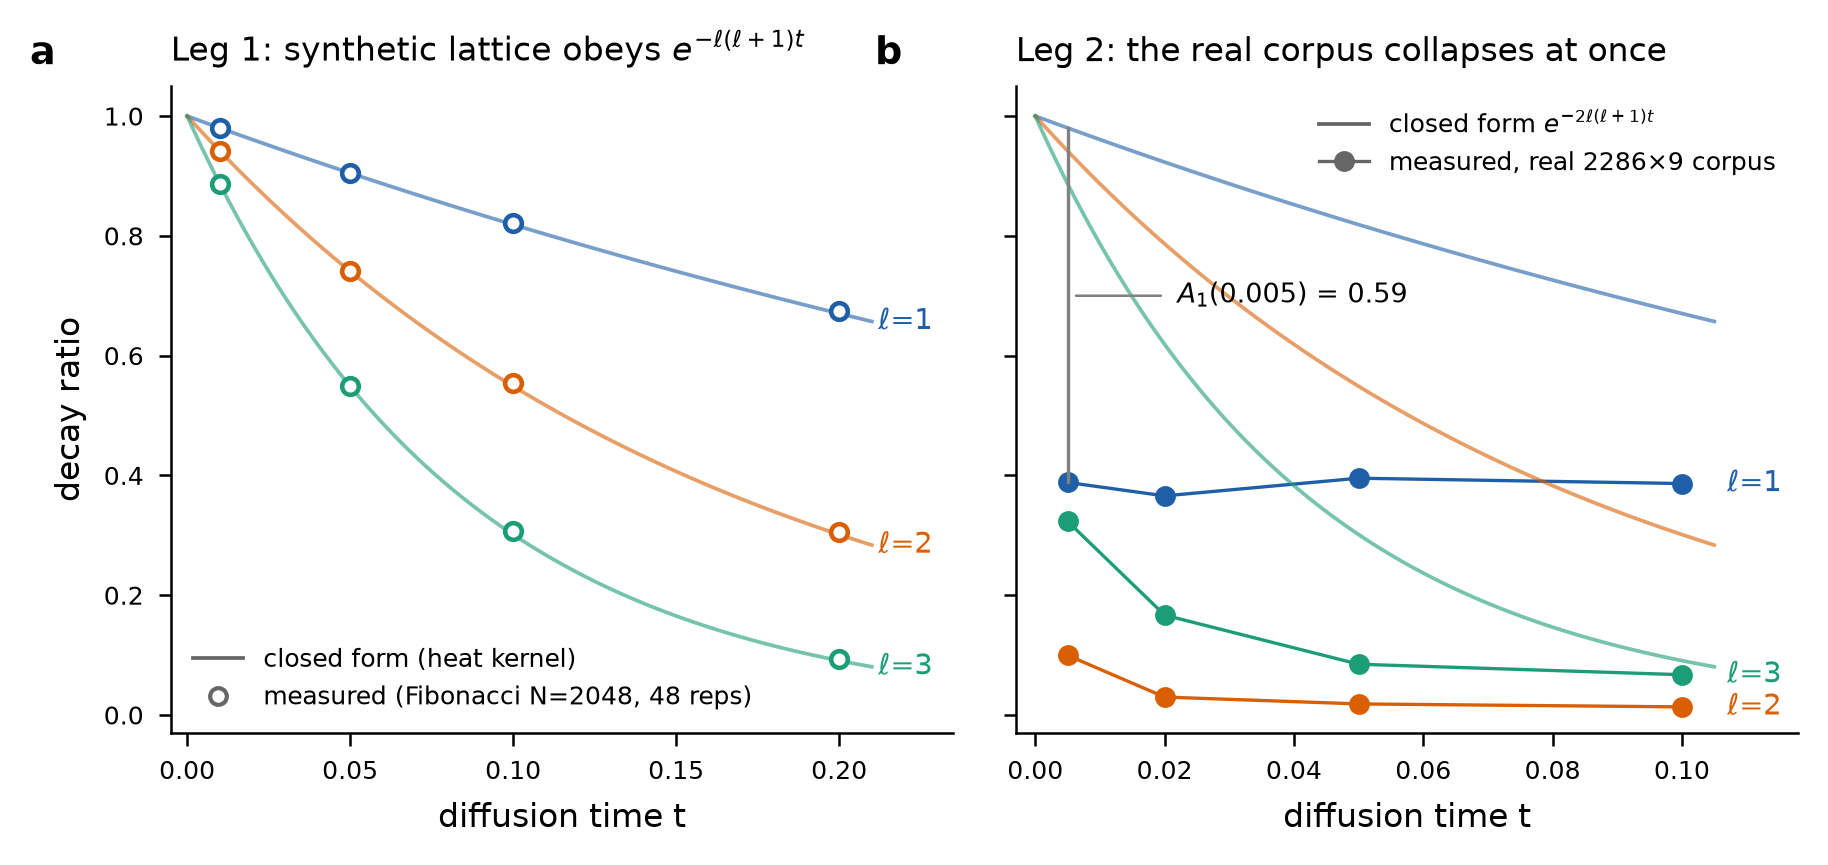
\includegraphics[width=\linewidth]{curvedcorpus_g1_defocus.png}
\caption{Experiment G1 spherical defocus: Leg 1 (synthetic Fibonacci lattice vs.\ closed-form heat kernel $e^{-2\ell(\ell+1)t}$) and Leg 2 (real $2286\times9$ corpus point-diffusion decay with atomicity diagnostic $A_1(0.005)\approx0.59$ marked). Source: \texttt{papers/data/g1/g1-results.json}.}
\label{fig:g1-defocus}
\end{figure}

The energy collapses at $t=0.005$ (RMS geodesic displacement ${\approx}0.14$ rad) where the closed form permits at most $6\%$ loss; the decay is non-monotone in $\ell$ ($\ell=3$ outlives $\ell=2$ at every $t$), impossible for heat-kernel decay of a smooth field; and a floor persists ($\ell=1$ stabilizes near $0.39$). The mechanism is the corpus's atomicity: only $176$ distinct rows of $512$ possible, so the point cloud is a set of heavy point masses, the fitted energy is carried by atomic coincidences rather than smooth harmonic structure, and an infinitesimal diffusion splits each atom into a cloud and kills the coherent fit. Leg 1 pins the identity; Leg 2 measures where its hypothesis (quasi-uniform design) fails. The gap is promoted to a diagnostic,
\begin{equation}
A_\ell(t)\;=\;e^{-2\ell(\ell+1)t}-\frac{E_\ell(t)}{E_\ell(0)},\tag{10}
\end{equation}
large at small $t$ iff the corpus's spherical energy is atomic ($A_1(0.005)\approx0.59$ on yubiOS). This is the same fact the Hodge channel reached through $176$ distinct rows and marginal dominance, now as one scalar; and it gates the generative extension: a Riemannian score-based model of this corpus must smooth the atoms first (vMF bandwidth as pre-diffusion) or it will model point masses. $A_\ell(t)$ \emph{was admitted to trial and failed} (v2, 2026-08-22): its null --- the same quantity on curveball draws, which share the atom structure of the marginals --- is now executed ($n{=}50$ draws, two seeds). The real $A_1(0.005)=0.945$ sits only $+1.3$--$+1.6$ null-SD above a null that is itself atomic (null mean $\approx 0.86$), so $A_1$ is marginal-dominated: a valid \emph{diagnostic} of atomicity, not an admissible corpus-specific map coordinate. Value-level vMF smoothing cannot halve it at any bandwidth $\kappa\in[2,1000]$ --- the 795-row all-ones atom is a point mass no kernel can spread. The verdict is recorded in \texttt{data/atomicity/A1-admission-null.json} and the repository CI now \emph{asserts the negative reproduces} (exit nonzero on drift in either direction).

\subsection{What the channel adds to the map}
(i) A scale-space: $z(t)$ profiles for every coordinate, corpus and null diffused identically, with the ultra-small-$t$ de-atomization window as the informative regime for atomic corpora. (ii) The slerp fold: geodesic rungs $\mathrm{slerp}(p_0,p^*;t_k)$ replace the log-odds amplitude ladder, making the fold intrinsic and composable with the achromatic Parseval coordinates. (iii) A generative standard-candle v2 by reverse diffusion, gated on de-atomization. (iv) A single knob unification: the Schr\"odinger bridge between null and corpus interpolates entropic diffusion ($T>0$) and optimal transport ($T\to0$), the same $T$ the compass swept on the $k$-marginal.

\section{Machine-checked invariants (Lean 4)}
\label{sec:lean}

The 2026-08-12 paper drew a boundary between identities (true by construction, carrying no data) and measurements, and showed the program had repeatedly mistaken one for the other. That boundary is now itself machine-checked. The file \texttt{CurvedCorpus.lean} (core Lean~4 toolchain, no \texttt{mathlib}) states and proves:

\begin{enumerate}
\item \texttt{atom\_delta\_nonneg} --- Lemma~1 in abstract form: the geodesic-only argmin over candidates including the stay option satisfies $\Delta=d_{\mathrm{pre}}-\min(\cdot)\ge0$.
\item \texttt{corpus\_sum\_nonneg} --- Theorem~1: a sum of non-negative per-file deltas is non-negative.
\item \texttt{cumulative\_monotone} --- Corollary~1: appending a non-negative per-cycle increment never decreases the running total.
\item \texttt{gate\_rank\_identity} --- C2's equivalence $V_2\ge2/5\iff2/V_2\le5$ in fraction form ($5p\ge2q\iff2q\le5p$ for positive $p,q$): provable by linear arithmetic alone, which is the formal content of ``the gate--rank equivalence carries no empirical information.''
\item \texttt{phi\_ladder\_telescope} --- D3's identity: $\sum_{k<n}\big(\Phi(k)-\Phi(k{+}1)\big)=\Phi(0)-\Phi(n)$; cumulative $\Delta$ telescopes by construction, not by discovery.
\item \texttt{heat\_exponent\_monotone}, \texttt{heat\_exponent\_additive} --- $\ell\mapsto\ell(\ell+1)$ is monotone and the exponent is additive in $t$: higher degrees always defocus faster (Eq.~(9)), and $e^{t\Delta}$ is a semigroup.
\item \texttt{mh\_flux\_symm} --- the $\min$-symmetry $\min(\pi_kq_{kk'},\pi_{k'}q_{k'k})=\min(\pi_{k'}q_{k'k},\pi_kq_{kk'})$, which is the algebraic core of Metropolis--Hastings detailed balance for the compass chain: both directed fluxes equal the same $\min$, so they balance identically.
\end{enumerate}

These are deliberately the \emph{identity-type} statements: nothing empirical is provable, and formalizing the identities is precisely how their non-empirical status is certified. The Monte-Carlo results (Tables~\ref{tab:leg1}--\ref{tab:leg2}, the calibration sweeps, the null tables) remain measurements with reproduction scripts, not theorems. The formalization uses integers and rationals-as-fractions with a hand-rolled \texttt{imin} so that no external mathematics library is required; each statement is closed by \texttt{omega}, structural induction, or definitional unfolding.

\section{Scope and honest caveats}
\label{sec:scope}

\textbf{Inherited.} Every caveat of the 2026-08-12 paper stands: the retraction is part of the record; $z$ is over-dispersed by roughly a third (nothing between $|z|=2$ and $4$ is decisive); Hodge magnitudes are construction-dependent; the sensitivity floor is $s\approx1$ log-odds at $N\le512$; the real-GWTC $z=+67$ certifies parameter redundancy, not astrophysics; azimuthal claims remain unsupported on real data, with the $m{=}3$ shares below their nulls for a stated mechanism.

\textbf{Optical language.} The identifications of Section~\ref{sec:optics} are exact only where stated: conformal maps and index profiles (geometrical optics regime; wave effects out of scope), Fermat/geodesic equivalence (stationarity, not global minimality; caustics excepted), lensing-as-null-standardization (a formal correspondence of measurement conventions, not a physical claim). There is no general theorem that data exhibits optical caustics; the caustic identification here is confined to the rank-degeneracy cases where the design map provably degenerates. ``Refractive index,'' ``focus,'' and ``caustic'' are not coordinates of the map and do not enter verdicts. One naming collision must be flagged before aberration language enters the program: the Zernike mode $Z_2^0$ is literally called ``defocus'' in optics, but it is a deterministic quadratic rephasing of the pupil---a focal-plane shift---whereas this paper's spherical defocus is stochastic heat flow in $t$. They are different objects sharing a word, and conflating the two would corrupt the optical dictionary rather than extend it (cf. \texttt{refs/zernike-fit-2026-08-24.md}). Should Zernike aberration coordinates ever be admitted, they face the membership condition exactly like every other coordinate---optical pedigree buys no exemption from it.

\textbf{Diffusion channel.} Leg 1 verifies the semigroup identity on the sampling lattice; it does not validate any corpus claim. Leg 2's atomicity diagnostic is specified with its null but the null leg is not executed, so $A_\ell(t)$ is not yet admissible. Diffusion time $t$, like the compass temperature $T$, is a knob of designed dynamics, not an observable of the corpus; no estimator of a ``corpus diffusion time'' is offered, and the $\hat t$ coordinate proposed in Section~\ref{sec:defocus} awaits its null. The Langevin extension of the compass is designed dynamics on the measured ladder; it does not reopen any equilibrium reading of the historical log ($0/598$ is untouched).

\textbf{Lean formalization.} The Lean file certifies identity-type statements only, over exact arithmetic (integers, fraction pairs); it does not formalize real analysis on $S^2$, the heat kernel, or any probabilistic statement, and it makes no claim about floating-point behavior of the shipped Python. The abstraction boundary is stated in the file header per theorem.

\textbf{Single-corpus caveats.} The matched-parameter ablation remains single-seed; the second-corpus re-run remains the open item of the predecessor. G1 Leg 2 is one corpus; the atomicity mechanism predicts the same collapse on any corpus with heavy row multiplicity, and that prediction is testable on the CIS/SCAP corpora already in the bundle.

\section{Addendum (v2, August 22, 2026): the lens, powered}
\label{sec:gapd-v2}

Every run of this program through v1 froze $\varphi_\theta$ at the identity. Gap D asked what happens when the 6 real degrees of freedom are optimized, subject to the anti-caustic guard (design rank $16$, condition number $\le 10^3$). It is now executed end-to-end in repository CI; all numbers below are seeded, deterministic, and recorded under \texttt{data/gapD/}.

\subsection{Synthetic target: the effect is real, its magnitude is a distribution}
On the planted $\ell{=}3$ family (amplitude $s{=}1$, $N{=}512$), a 15-seed sweep of the canonical script gives $\Delta J \in [+0.40, +7.73]$ null-SD (median $+3.22$, mean $+3.33 \pm 2.01$); the pre-registered bar $\Delta J > 2$ clears in $11/15$ seeds. At $6\times$ optimizer budget, 3 of the 4 sub-bar seeds flip ($14/15$ total): the misses were optimizer starvation, not absence of effect. The amplitude sweep $s \in \{0.25, \dots, 2\}$ shows no threshold where the effect dies, and resolves the residual failures as \emph{headroom}: $\Delta J$ anticorrelates with the identity chart's own $J$ --- when the frozen chart already captures the signal, no lens can add two null standard deviations (the one persistent holdout flips to $+5.71$ at $s{=}0.25$, exactly where its identity $J$ collapses).

\subsection{The real corpus behind its matched null}
The first lens run on the real $2286\times 9$ corpus (PC1/PC2 sphere lift, PC3 field, the documented defocus convention; null $=$ 20 curveball draws through the identical pipeline; guard enforced on the real \emph{and} every null design): at the identity chart the real corpus's $\ell{=}3$ energy share sits \emph{below} its fixed-margin null ($J = -1.51$; share $0.031$ vs $0.074 \pm 0.028$). The optimized chart reaches share $0.408$ against a null collapsed to $0.0345 \pm 0.0030$: $\Delta J = +126.1$. Because the lens is optimized on the real data, the honest comparator is a \emph{selection null}: optimizing a lens for each of 10 curveball draws treated as the target, under identical selection pressure, yields $\Delta J$ median $+5.1$, max $+25.5$. The real corpus is $\approx 4.9\times$ the strongest control --- the result is not an optimization artifact. There is corpus-specific $\ell{=}3$ structure beyond the margins, and it is visible \emph{only under a non-identity chart}. This is complementary to the $A_\ell$ verdict above: admission is chart-dependent --- the coordinate that fails under the frozen chart is precisely what the powered lens separates.

\subsection{Geometry of the optimized chart}
Normalized to $ad - bc = 1$: $a = 1.4387 + 0.3249i$, $b = -0.1220 + 0.4316i$, $c = -0.0442 - 0.5509i$, $d = 0.8293 - 0.1538i$. The trace is $2.268 + 0.171i$, $\mathrm{tr}^2 = 5.115 + 0.776i \notin [0,4]$: the transformation is \emph{loxodromic}, with multiplier $|\lambda| = 2.924$ (translation length $\log|\lambda| = 1.073$) and rotation $\arg\lambda = 17.5^{\circ}$ --- a spiral zoom. Its attracting fixed point lifts to $(-0.437, 0.749, 0.498)$ on $S^2$ and its repelling fixed point to $(-0.132, -0.758, -0.639)$; the pole $-d/c$ (the point of maximal magnification) lifts to $(-0.095, -0.912, 0.399)$. The optimized design's condition number is $997.8$ against the guard cap of $10^3$, and $155/471$ candidate evaluations were guard-rejected: the optimizer converged \emph{onto the anti-caustic boundary}. The best admissible lens is the most extreme admissible lens --- maximal magnification short of a caustic, aimed so as to stream the corpus embedding from the repelling point toward the attracting point while rotating it $17.5^{\circ}$ per unit flow. In the optical vocabulary of Section~4, lens design did not find a gentle refinement: it found the rim of the permitted design space. Numbers: \texttt{data/gapD/lens-geometry-2026-08-22.json}.

\subsection{Loxodromic navigation (executed same day)}
The optimized chart's loxodromic structure was used three ways (pre-registered; \texttt{data/gapD/loxodromic-navigation-2026-08-22.json}; script \texttt{scripts/gapD\_loxodromic\_navigation.py}). \emph{(i) Flow trace.} $M$ has canonical fractional powers $M^t$; tracing $J(t)$ for $t \in [0, 1.5]$ (step $0.05$, same seed and null draws) gives a \emph{perfectly monotone} ascent (Spearman $\rho = 1.0$ on $[0,1]$): $J$ rises from $-1.51$ at the identity, crosses zero near $t \approx 0.5$, and reaches $+124.6$ at $t = 1$ (reproducing the recorded optimum); the anti-caustic guard fails at $t = 1.05$. The discrete 8-parameter optimum is therefore the \emph{boundary point of its own one-parameter flow}: lens design on this corpus reduces to navigation --- choose the loxodromic bearing, sail toward the caustic at constant heading, stop at the rim. \emph{(ii) Mercator chart.} Conjugating the fixed points to $0$ and $\infty$ linearizes the lens ($\zeta \mapsto \kappa\zeta$, $|\kappa| = 0.342 = 1/|\lambda|$) and assigns every row flow coordinates $(u, v)$; the phase $v$ is nearly uniform (circular $R = 0.063$) and the flow time $u$ correlates $\rho_s = 0.48$ with the row margins. \emph{(iii) Admission.} Per the membership condition, $\mathrm{sd}(u)$ faced the curveball null and \emph{failed}: $z = +1.64 < 3$. The flow coordinate joins $A_1$ among the rejected: no scalar summary so far survives the fixed-margin trial --- the corpus-specific signal lives in the optimized lens functional itself, not in any single coordinate it induces.

\emph{Caveats.} The $+126.1$ is large partly because $J$ standardizes by a null SD the optimizer itself compresses; the selection-null factor ($\approx 5\times$) is the defensible effect size. PC3-as-field is a documented convention of the defocus deliverable, not dictated by the papers. The optimizer is small-budget random search: every $\Delta J$ here is a lower bound.

\section{Addendum (August 24, 2026): corpus sonometry, and two gaps closed}
\label{sec:sonometry}
Three additions land after v2, machine-checked in \texttt{CurvedCorpus.lean} (sections~10--12) and executed in CI beside it (\texttt{verify\_claims.py} claims~7--8; instrument \texttt{tools/corpus-sonometer}).

\textbf{(i) F3 canonicity, closed.} Uniqueness-from-irreducibility, previously cited as outside machine reach, is now proved in core Lean (\texttt{stationary\_unique\_uniform}, section~10) via the discrete maximum principle: on an irreducible fibre, every stationary weight vector of a nonnegative symmetric constant-row-sum kernel is constant, so the uniform distribution is \emph{the} stationary law of the curveball chain. Claim~6 continues to discharge irreducibility exhaustively on the test instance.

\textbf{(ii) The Lyu--Mukherjee anchor, split.} The Marchenko--Pastur target moments are Narayana polynomials $m_k(\lambda)=\sum_r N(k,r)\,\lambda^r$ (sums over non-crossing partitions weighted by block count). Section~11 proves the rows through $k=8$ and their Catalan row-sum specialization $m_k(1)=C_k$ as exact kernel-checked identities, via the free-Poisson functional equation $M = 1 + zM(M+\lambda-1)$; claim~7 measures the curveball-sampled constant-margin ensemble's empirical spectral moments against them ($n{=}512$, $p{=}128$, $\lambda{=}0.25$; relative error $\le 0.5\%$ for $k\le4$). The weak-convergence limit statement itself remains cited, per the scope discipline.

\textbf{(iii) The corpus level, in dBc.} Effects are now also reported on a decibel-style level scale referenced to the vacuum:
$L \;=\; 20\log_{10}\!\left(\frac{|\Delta V_2|}{\sigma_{\mathrm{null}}}\right)\ \text{dBc},$
so that $0$~dBc is the null ensemble's own RMS fluctuation --- the smallest detectable effect, the acoustician's $20\,\mu$Pa. The published $z=+12.13$ reads $+21.7$~dBc; CI measures $+24.3$~dBc at the 20N mixing window and $+17.4$~dBc at 40N, both far above the $+15.6$~dBc detectability floor ($z>6$). The level laws that make the scale meaningful --- cascade additivity (gains multiply, levels add; the discrete form of the heat-exponent additivity of Section~\ref{sec:defocus}), the pressure/power factor of two ($20\log_{10}$ versus $10\log_{10}$ is exact, not conventional), strict monotonicity and injectivity --- are proved as exact identities on integer powers in section~12; the real-valued $\log_{10}$ stays on the measurement side of the boundary.

\section{Addendum (September 1, 2026): the phonon reading}
\label{sec:phonons}
The acoustic/optical phonon vocabulary is placed against the program the same way the photophysics families were (refs bridge, 2026-08-25): exclusion-only verdicts, parameter parsimony as the binding gate. Full accounting in \texttt{refs/acoustic-optical-phonons-bridge-2026-09-01.md}; instrument \texttt{tools/phonon-dispersion}; identities in \texttt{CurvedCorpus.lean} section~14. Four results are load-bearing.

\textbf{(i) The acoustic sum rule is the $\ell=0$ conservation law --- and the Goldstone reading is excluded.} In a harmonic lattice the force-constant matrix annihilates the uniform translation, which is why the acoustic branch is exactly gapless at the zone center; in the program the defocus generator annihilates the constant function, which is why $E_0$ is conserved and the forward flow terminates at uniform. That constraint-structure identity is proved term by term (\texttt{acoustic\_sum\_rule}). The stronger Goldstone reading fails: no spontaneously broken symmetry, no order parameter, and on a compact $S^2$ no gapless continuum --- the spectrum is one conserved mode plus gapped modes, $\lambda(\ell) = 2\ell(\ell+1) \in \{0, 4, 12, 24, \dots\}$. Consequently the program has \emph{no optical branch either}: a second branch requires a second population per site (two atoms per cell), and the delayed/prompt split ($0.9774$ vs $0.2059$ spectral mass) is a cut on one branch, not a second one. The zone-boundary algebra that would open a diatomic gap is nonetheless kernel-checked --- $(a{+}b)^2 - 4ab = (a{-}b)^2$, gap open iff the masses differ (\texttt{diatomic\_disc}, \texttt{gap\_closes\_iff}) --- against the day a two-population (partially exchangeable) extension is admitted; note the natural split, the 795 saturated rows, is margin-determined and has curveball deflection exactly zero.

\textbf{(ii) Klemens replaces $k_{\mathrm{ISC}}$: selection rules instead of a fitted matrix.} The photophysics bridge proposed inter-$\ell$ transfer via a generic non-normal coupling $K_{\ell\ell'} = k_{\mathrm{ISC}}\,\mathbf{1}[\ell' > \ell]$, $O(L^2)$ free entries. The phonon literature has owned this process since 1966: an optical quantum decays anharmonically into two acoustic quanta, conserving energy and momentum (Klemens, \emph{Phys.\ Rev.}\ 148, 845). Transcribed to $S^2$, cubic anharmonicity couples degrees only through Gaunt coefficients, which vanish unless $|\ell_1-\ell_2| \le \ell_3 \le \ell_1+\ell_2$, $\ell_1+\ell_2+\ell_3$ even, $m_1+m_2+m_3 = 0$ --- the rotational analogue of $q_1+q_2+q_3=0$. The sparsity pattern is derived, not fitted; one amplitude $\kappa$ remains. At the working truncation $L=3$ the structure is not vacuous: of $64$ triads, $23$ survive ($41$ forbidden, $64\%$), kernel-checked by enumeration and cross-checked against the exact Wigner $3j(\ell_1\ell_2\ell_3;000)$ zero pattern and the Simpson triple-Legendre integral. The energy side is exact integer arithmetic: on the diatomic chain the channel closes iff the mass ratio exceeds $3$ (\texttt{klemens\_condition}). The generic $k_{\mathrm{ISC}}$ matrix is excluded in favour of the Gaunt-structured coupling before either is fitted; the transient-growth prediction (a corpus transiently \emph{more} structured under defocus) survives unchanged, and if non-monotone $E_\ell(t)$ is ever measured, phonon hydrodynamics (second sound) is the named prior art.

\textbf{(iii) The occupation statistics are Fermi--Dirac, not Bose--Einstein.} The primitives are two-state sites, so at linear $\Phi(k) = \varepsilon k$ the compass stationary law is exactly $\pi_T(k) = \binom{9}{k} p^k (1-p)^{9-k}$ with $p = 1/(1+e^{\varepsilon/T})$ --- the FD occupancy, zero new parameters, machine-precision verified. The BE identity is excluded (bounded $k$, no multiple occupancy, explicit $\binom{9}{k}$ degeneracy). The residual between the measured $\Phi(k)$ and its linear reference is a parameter-free ``interaction beyond the ideal two-state gas'' readout; it faces its own curveball admission null before it becomes a statistic. Designed-chain wall throughout: these are compass properties.

\textbf{(iv) The corpus's native spectrum is the Hamming graph's; $S^2$ is its continuum idealization.} A $\{0,1\}^9$ corpus decomposes exactly over $H(9,2)$: Laplacian eigenvalue $2j$ at Hamming weight $j$, multiplicity $\binom{9}{j}$, Krawtchouk polynomials playing Legendre's role (both are Gelfand-pair harmonic decompositions). The heat kernel there decays \emph{linearly} in level, $e^{-2jt}$, against the sphere's quadratic $e^{-2\ell(\ell+1)t}$; beyond the shared zero mode the sphere penalizes level strictly faster ($\ell < \ell(\ell+1)$ for $\ell \ge 1$, \texttt{heat\_exp\_dominates\_hamming}). Any cross-basis comparison of fitted timescales inherits the C1 discipline. Two further verdicts close the sweep: Lyddane--Sachs--Teller and LO--TO splitting are \emph{void} (no vector field, no polar mode, no $\varepsilon(\omega)$; the lens factor $|\varphi'_\theta|^2$ is a Jacobian, not a response kernel), and phonon transport is \emph{void} (the generator is diagonal; nothing propagates --- $\mathrm{d}\lambda/\mathrm{d}\ell$ is not a group velocity). The Pennes $\omega$ of the photophysics addendum is re-read as a mass term gapping the whole spectrum uniformly, and thereby demoted: every currently admitted statistic is a ratio, invariant under $E \mapsto e^{-\omega t}E$, so $\omega$ is unidentifiable until an unnormalized observable is admitted.

\section{Conclusion}
\label{sec:conclusion}

Merged, the program reads as one arc. An instrument was built (curves, atom, loop) whose invariants are real but whose headline statistics were, to first order, properties of its own marginals and bases; an audit rebuilt it around a null-standardized question space with exclusion-only verdicts; and the present paper closes the loop twice over. Downward, into certified algebra: the identity-type claims are now Lean-checked, so the line between what the program \emph{proves} and what it \emph{measures} is mechanical. Outward, into dynamics: the frozen M\"obius chart is recognized as a conformal lens --- unpowered in v1, powered and measured in v2 (Section~\ref{sec:gapd-v2}), the null space as the $t\to\infty$ endpoint of a heat flow that is diagonal in the program's own basis, and the historical absorbing edit log as the zero-temperature corner of a sphere Langevin whose deterministic half is slerp. The semigroup law is verified where its hypotheses hold; where they fail, the failure is measured, named ($A_\ell(t)$, atomicity), and put behind the same membership condition as every other coordinate. Focusing a feature space, in this vocabulary, is now a concrete open problem with a concrete guard: power the lens (optimize $\varphi_\theta$ under a null-standardized objective), and never let it reach a caustic.

\section*{References}

\noindent S.~Tchatalbachian. Learned latent curves and the hyperspherical-harmonic variant: a closed-loop framework for corpus embedding and recursive skill auditing. Internal paper, \texttt{papers/learned-latent-curves-2026-08-06.tex}, 2026a.

\medskip\noindent S.~Tchatalbachian. Is this $X$? A null-standardized question space for corpus curvature, with a Hodge-theoretic channel and a calibrated standard-candle generator. Internal paper, \texttt{papers/is-this-x-2026-08-12-Final.tex}, 2026b.

\medskip\noindent U.~Leonhardt. Optical conformal mapping. \emph{Science} 312:1777--1780, 2006.

\medskip\noindent M.~Schmiele, V.~S. Varma, C.~Rockstuhl, and F.~Lederer. Designing optical elements from isotropic materials by using transformation optics. \emph{Physical Review A} 81:033837, 2010.

\medskip\noindent R.~Kalaba and S.~Ueno. Dynamic programming, Fermat's principle and the eikonal equation. \emph{JOSA} 64(3):317, 1974.

\medskip\noindent T.~Tyc. Fermat's principle and the general eikonal equation in a static anisotropic medium. \emph{JOSA A} 14(10):2850, 1997.

\medskip\noindent C.~R. Rao. Information and the accuracy attainable in the estimation of statistical parameters. \emph{Bull.\ Calcutta Math.\ Soc.} 37:81--91, 1945.

\medskip\noindent N.~N. \v{C}encov. \emph{Statistical Decision Rules and Optimal Inference.} AMS Translations of Mathematical Monographs 53, 1982.

\medskip\noindent B.~Efron. Defining the curvature of a statistical problem. \emph{Annals of Statistics} 3(6):1189--1242, 1975.

\medskip\noindent V.~A. Marchenko and L.~A. Pastur. Distribution of eigenvalues for some sets of random matrices. \emph{Mat.\ Sbornik} 72(4):507--536, 1967.

\medskip\noindent H.~Lyu and S.~Mukherjee. Large random matrices with given margins. arXiv:2407.14942, 2024.

\medskip\noindent S.~Dasgupta and A.~Gupta. An elementary proof of a theorem of Johnson and Lindenstrauss. \emph{Random Structures \& Algorithms} 22(1):60--65, 2003.

\medskip\noindent T.~Zhang. Learning bounds for kernel regression using effective data dimensionality. \emph{Neural Computation} 17(9):2077--2098, 2005.

\medskip\noindent K.~Shoemake. Animating rotation with quaternion curves. \emph{SIGGRAPH} 19(3):245--254, 1985.

\medskip\noindent T.~White. Sampling generative networks. arXiv:1609.04468, 2016.

\medskip\noindent V.~De Bortoli, E.~Mathieu, M.~Hutchinson, J.~Thornton, Y.~W. Teh, and A.~Doucet. Riemannian score-based generative modelling. \emph{NeurIPS}, 2022.

\medskip\noindent C.-W. Huang, M.~Aghajohari, J.~Bose, P.~Panangaden, and A.~Courville. Riemannian diffusion models. \emph{NeurIPS}, 2022.

\medskip\noindent A.~Lou et al. Scaling Riemannian diffusion models. \emph{NeurIPS}, 2023.

\medskip\noindent L.~Ambrosio, N.~Gigli, and G.~Savar\'e. A user's guide to optimal transport. Lecture notes, 2011.

\medskip\noindent G.~Strona, D.~Nappo, F.~Boccacci, S.~Fattorini, and J.~San-Miguel-Ayanz. A fast and unbiased procedure to randomize ecological binary matrices with fixed row and column totals. \emph{Nature Communications} 5:4114, 2014.

\medskip\noindent X.~Jiang, L.-H. Lim, Y.~Yao, and Y.~Ye. Statistical ranking and combinatorial Hodge theory. \emph{Mathematical Programming} 127(1):203--244, 2011.

\medskip\noindent H.~Vogel. A better way to construct the sunflower head. \emph{Mathematical Biosciences} 44:179--189, 1979.

\appendix

\section{Reproduction manifest (delta over prior bundles)}
\label{app:manifest}

New artifacts of this paper (session bundle, seed $20260813$): \texttt{g1/g1\_defocus.py} (both G1 legs; numpy only; ${\sim}3$ min), \texttt{g1/g1-results.json} (full record of Tables~\ref{tab:leg1}--\ref{tab:leg2}), \texttt{refs/spherical-defocus-g1-2026-08-13.md} (the G1 refs note), \texttt{lean/CurvedCorpus.lean} (the seven machine-checked statements of Section~\ref{sec:lean}; core Lean~4, no \texttt{mathlib}). Input data: \texttt{data/real/per\_row\_coverage\_v3.json} from the shipped \texttt{is-this-x} evidence bundle (2286 rows; column sums as in its Appendix A). Everything else --- the curveball samplers and their uniformity proofs, the ladder, the candle, the Hodge decomposition, the compass --- is unchanged and lives in the two prior bundles under their own manifests.


\medskip\noindent \textbf{v2 delta (2026-08-22).} \texttt{scripts/gapD\_lens\_power.py} (canonical Gap D, executed: 15-seed sweep + budget + amplitude), \texttt{scripts/gapD\_real\_corpus\_lens.py} (real-corpus lens + selection-null control), \texttt{data/gapD/seed-sweep-2026-08-22.json}, \texttt{data/gapD/followups-2026-08-22.json}, \texttt{data/gapD/lens-geometry-2026-08-22.json}, \texttt{data/atomicity/A1-admission-null.json} (the executed $A_\ell$ admission null; CI-enforced recorded negative), the inverted \texttt{--admit-null} CI gate in \texttt{lean-check.yml}, \texttt{scripts/gapD\_loxodromic\_navigation.py}, and \texttt{data/gapD/loxodromic-navigation-2026-08-22.json}.

\end{document}
